\section{\emph{lemon} and UBY-LMF}
\begin{figure}
 \begin{center}

 	 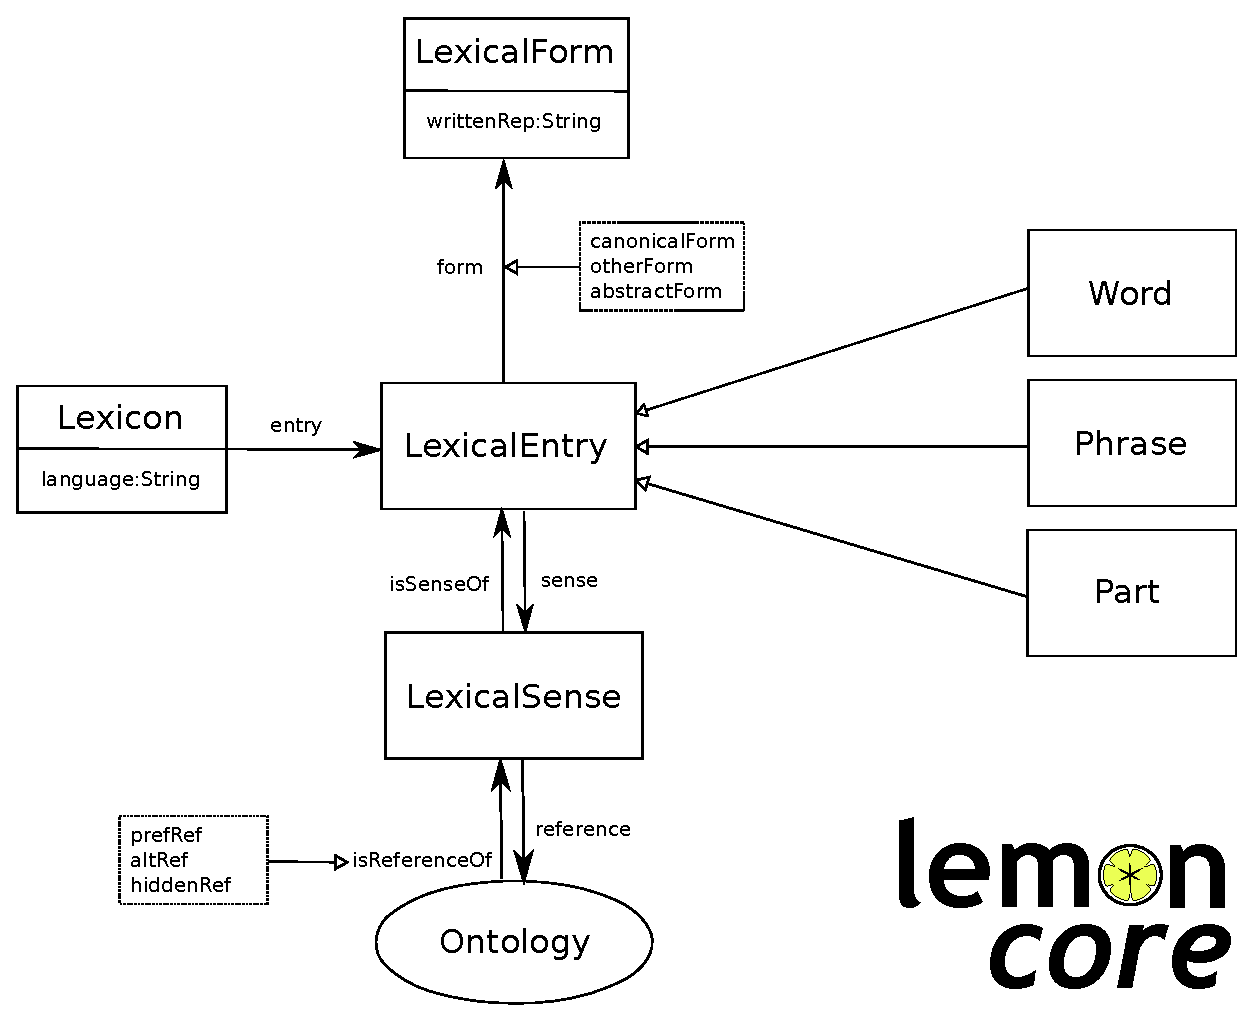
\includegraphics[width=1.0\columnwidth]{images/lemon-core}

 \end{center}
\caption{The core of the \emph{lemon} model\label{lemon-core}}
\end{figure}

The \emph{lemon} model\cite{mccrae2012interchanging} is a  lexicon model for representing and sharing ontology lexica.
It supports publishing 
lexical-semantic resources as linked data on the basis of the following principles:

\begin{description} 
\item[LMF-based:]{To allow easy conversion from non-linked data resources.}
\item[RDF-native:]{Publishing as linked data, with RDFS and OWL used to describe
  the semantics of the model.}
\item[Modular:]{Separation of lexicon and ontology layers, so that \emph{lemon} lexica can be linked to existing ontologies
in the linked data cloud.}
\item[Externally defined data categories:]{Linking to data categories in
  annotation terminology repositories, rather than being limited to a specific part-of-speech tag set.}
\item[Principle of least power:]{The smaller the model and the less expressive the language, 
	the wider its adoption and the higher the reusability of the
	data\cite{shadbolt2006semantic}.}
\end{description}

This \emph{lemon} core model is illustrated in Fig.\ \ref{lemon-core}, which defines the
basic elements used by all lexica published as linked data. In addition to this, there
are a number of modules used to model linguistic description, syntax, morphology 
and relationships between lexica.\footnote{More details on the model and descriptions of
the modules can be found at \url{http://lemon-model.net}}

%UBY is both a network of interlinked lexical-semantic resources 
%and a project on continuous integration and linking of lexical resources for NLP applications.
% It is motivated by the
%observation that an essential requirement in NLP is the availability of a wide range of lexical resources that can be used for many different NLP tasks. In a continuous process, such resources
%are integrated into UBY by means of (i) making them inter-operable  and (ii)
%linking them to other resources in UBY at the sense level.

%UBY has currently integrated 10 LRs in two languages, see www.ukp.tu-darmstadt.de/uby. Only 8 of these LRs have open licenses and 
%can be offered as a UBY database dump for download: English WordNet, Wiktionary, Wikipedia, FrameNet and VerbNet, German Wikipedia, Wiktionary, and multilingual OmegaWiki. 
%A subset of these LRs is linked at the word sense level and these sense alignments are open as well. 
%There are monolingual sense alignments between VerbNet--FrameNet\footnote{\url{http://verbs.colorado.edu/semlink/}} and 
%VerbNet--WordNet\footnote{\url{http://verbs.colorado.edu/~mpalmer/projects/verbnet}} as well as between WordNet--Wikipedia \cite{niemann2011peoples} and WordNet--Wiktionary  \cite{meyer2011what}. In addition, Uby provides cross-lingual sense alignments between WordNet and the German OmegaWiki \cite{gurevych2012uby}, also including the inter-language links already given in Wikipedia and OmegaWiki.
%
%UBY databases can be created according to specific application needs: a user might want to use only a subset of the LRs integrated into UBY, convert them to UBY-LMF and import them into
%a database. Any UBY database can be accessed with a single Java-API which is continuously developed along with the conversion tools in an Open Source Project on Google Code (code.google.com/p/uby).
%UBY and UBY-LMF are CC-licensed and the UBY-related software is licensed under the open Apache license. 

In UBY, interoperability is achieved by standardizing lexical resources according to UBY-LMF \cite{ecklekohler2012uby,TUD-CS-2013-0003}, a lexicon
model which is a full-fledged instantiation of the ISO standard LMF, specifically for NLP.
%instantiates the Lexical Markup Framework (LMF, ISO 24613:2008, \cite{francopoulo2006lexical}). 

In comparison to the \emph{lemon} lexicon model,  UBY-LMF is similar in two aspects: first it is LMF-based, and second,
it uses externally defined data categories from
ISOCat.\footnote{\url{http://www.isocat.org/rest/dcs/484}}
In contrast to \emph{lemon}, however, UBY-LMF is based on two quite different principles:
\begin{description} 
\item[Principle of Adoption:]{UBY-LMF has been designed to fully cover a wide range of heterogeneous lexical resources
without information loss.}
%This resulted  in a fine-grained model of lexical information types, which ranges from morphology and lexical syntax to lexical semantics and the mapping between syntactic and semantic arguments. 
\item[Independence of implementation:]{UBY-LMF  is independent of any particular implementation. There are many ways to implement an LMF lexicon model \cite{francopoulo2007lexical}, including RDF.} 
\end{description}


%UBY-LMF, is currently represented in two ways: first, as a DTD, and second, as a Java Object-Relational Mapping by means of the Hibernate framework\footnote{\url{http://www.hibernate.org}}, 
%which allows mapping any instance of UBY-LMF either to a SQL database or to an XML file.
%Both ways of representing UBY-LMF do not require the use of globally unique identifiers (URIs). 
%However, an implementation of UBY-LMF in RDF would be possible as well.
%, since UBY-LMF as such is independent of any particular implementation or 
%serialization and an LMF lexicon model can be implemented in many ways \cite{francopoulo2007lexical}.

% JEK I would not call it extension
%An extension of LMF to include URIs \cite{Francopoulo2007}, and full-fledged RDF linearizations of LMF have been suggested, e.g., in the context of the Lexicon Model for Ontologies (Lemon) as described by McCrae et al. (2011)\nocite{McCrae2011}.
%An implementation of LMF to include URIs has already been suggested\cite{francopoulo2007lexical}.
%In fact, providing lexical resources, in particular interlinked resources such as UBY, as linked data is a very natural
%step to take and
%allows us to integrate UBY-LMF-based resources with other resources previously converted to RDF. 
%e.g., in the context of the developing Semantic Web.

%, and full-fledged RDF linearizations of LMF have been suggested, e.g., 
%in the context of the Lexicon Model for Ontologies (Lemon) for a variant of LMF as described by McCrae et al. (2011)\nocite{mccrae2011linking}.
We performed a
mapping of UBY-LMF to \emph{lemon} which allows conversion of lexical resources in UBY-LMF format to \emph{lemon} format.
%Apart from the fact that the mapping of UBY-LMF to \emph{lemon} is an interesting task per se, because \emph{lemon} links lexical resources and 
%ontologies, there is another reason for this mapping. 
%The LMF standard is not an open standard (in the sense that its specification is not freely available), while \emph{lemon} provides an
%interchange format which fully complies with open data and open access principles.

%An extension of LMF to include URIs \cite{Francopoulo2007}, and full-fledged RDF linearizations of LMF have been suggested, e.g., in the context of the Lexicon Model for Ontologies (Lemon) as described by McCrae et al. (2011)\nocite{McCrae2011}.

%Originally, Uby was implemented using the Lexical Markup Framework, a standard aiming for interoperability among lexical-semantic resources.

% LMF is no format, it is an abstract standard
%First, the LMF standard is not an open standard (in the sense that its specification is not freely available), and,
% according to the experience of UBY, the application of the standard requires % making 
%NLP domain-specific modifications to the abstract model defined by the standard.
%Second, the currently used implementation of UBY-LMF does not consider how resources can be uniquely identified on the web. 


%and in its frequently used
% LMF does not say anything about serialization, XML is just an illustrative example
 %serialization as XML, it does not consider how resources can be uniquely identified on the web. 
%Furthermore, according to the experience of UBY, application of the standard requires % making 
%NLP domain-specific modifications to the standard schema.

%An RDF formalization tackles %of LMF allows us to tackle 
%some of these problems, and this has been suggested by the LMF developers themselves% \citep{francopoulo2009multilingual}
%.\footnote{\url{http://www.tagmatica.fr/lmf/LMF_revision_14_In_OWL29october2007.xml}}

%LMF is grounded in earlier research on feature structures (i.e., directed acyclic graphs) that have been suggested as a generalization over resource-specific data structures \citep{veronis-ide92-feature-structures-for-lexical-dbs}.
%Feature structures are a flexible and general formalism, which became the basis for subsequent standardization, in particular, in LMF.
%\citealp{francopoulo2006lexical}).

% LMF represents a metamodel % aiming to provide a standard 
% to represent semantic information in NLP lexicons and machine-readable dictionaries.
% It has been successfully applied to develop resources, including the different Uby data sets.

%Converting a lexical resource in UBY-LMF format to lemon requires a mapping of the UBY-LMF lexicon model to the lemon lexicon model. 

Although both UBY-LMF and \emph{lemon} are based on LMF, the mapping revealed substantial differences. These are mainly due to the fact that 
\emph{lemon} is a model for ontology lexica where the lexicon and ontology layers are kept separate. Thus, sense representations in \emph{lemon} primarily consist of references to the associated ontology
where a rich and domain-specific sense definition is provided. 
The development of UBY-LMF, on the other hand, has been driven by the requirement to cover a large variety of
 lexical information types, which ranges from morphology and lexical syntax to lexical semantics and the mapping between syntactic and semantic arguments. 
Thus, the resulting lexicon model makes use of very fine-grained sense specifications which are often grounded in linguistic theories.
%e.g. Frame Semantics (the basis of FrameNet) or the Levin alternation classes of verbs \cite{levin93} (the basis of VerbNet).


